\documentclass[12pt]{article}
\usepackage{xeCJK}%preamble part
\usepackage{graphicx}
\usepackage{indentfirst}
\usepackage[a4paper, inner=1.5cm, outer=3cm, top=2cm, bottom=3cm, bindingoffset=1cm]{geometry}
\usepackage{epstopdf}
\usepackage{listings}
\usepackage{array}
\usepackage{fontspec}
\usepackage{bm}
\usepackage{gensymb}
\usepackage{todonotes}
\usepackage{amsmath}
\usepackage[citecolor=blue]{hyperref}

\usepackage{makecell}
\usepackage[lofdepth,lotdepth]{subfig}




\setlength{\extrarowheight}{4pt}
\setlength{\parindent}{1cm}
\begin{document}
\title{\textbf{\fontsize{15.75pt}{\baselineskip}{讨论}}} 

\author{\fontsize{12pt}{\baselineskip}{数33 赵丰}}
\maketitle
\large
本次讨论以近可能简化的数学模型推导出FIM的结构,这个结构和之前一直研究的matrix结构是一致的。
先考虑非协作的情形(只研究平面定位),即定位场景中有$N_b$个anchor和$N_a$个移动节点anget,如下图所示:
\begin{figure}[!ht]
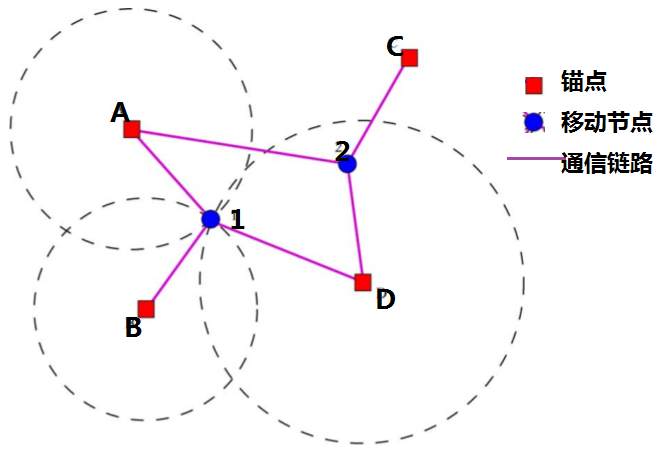
\includegraphics[width=\textwidth]{002.png}
\end{figure}

上图中红色的方框是锚点,而蓝色的圆圈是移动节点。由于是非协作的,每个移动节点的定位都可以分别考虑,anchor是位置已知的,记为$\{\bm{p}^b_1,\bm{p}^b_2,...\bm{p}^b_{N_b}\}$,待定位的移动节点的位置为$\bm{p}$,现在假设agent和每一个anchor都可以相互通信进行无线测距,得到的函数是$
f(||\bm{p}^b_i-\bm{p}||)$,f依赖于测量方式的不同,直接测距情形下是常数,$||\bm{p}^b_i-\bm{p}||$是$\bm{p}^b_i$和$\bm{p}$之间的欧式距离。
测角和测信号强度情形下都不一样。
假设每个测量都伴随有随机的高斯噪声,即测量的观测值是一个$f(||\bm{p}^b_i-\bm{p}||)$,方差为$\sigma$的正态分布$X_i$,对于$N_b$个锚点,可以得到$X_1,...X_{N_b}$的联合概率密度函数为$N_b$维的正态分布,且我们假设各个锚点和待测的移动节点的通信是独立的,所以$X_i$之间彼此独立,联合概率密度函数为:
\begin{equation}
f(x_1,...x_{N_b}|\bm{p})=\prod_{i=1}^{N_b}\frac{1}{\sqrt{2\pi\sigma^2}}exp(-\frac{(x_i-f(||\bm{p}^b_i-\bm{p}||))^2}{2\sigma^2}
\end{equation}
由此得到对数似然函数为(略去常数项):
\begin{equation}
\log(\Lambda)=\displaystyle\sum_{i=1}^{N_b} -\frac{(x_i-f(||\bm{p}^b_i-\bm{p}||))^2}{2\sigma^2}
\end{equation}
由FIM矩阵的定义,可以推出对其中一个移动节点,FIM是2行2列的对角阵:
\begin{equation}\label{eq:uu}
FIM=\displaystyle\sum_{i=1}^{N_b}\frac{f'^2}{\sigma^2}\bm{u}_i\bm{u}_i^T
\end{equation}
其中$\bm{u_i}=\frac{\bm{p}^b_i-\bm{p}}{||\bm{p}^b_i-\bm{p}||}$,是待测节点和第i个锚点的单位方向向量。在无线定位中$\bm{u_i}^T\bm{u_i}$前面的系数被叫做range information intensity(RII),通常用$\lambda_i$表示。可以看出,各个锚点对FIM的贡献以和式相加,其中building block是$\lambda_i \bm{u}^T\bm{u}$,这是一个奇异的矩阵,但2个不同方向的这种矩阵相加是非奇异的。在沈老师之前的文献中,用信息椭圆的方法给出了这种矩阵一种几何解释。

如果非协作定位场景中有$N_a$个移动节点,总的FIM是$2*N_a$维的矩阵,但由于各个节点之间相互独立,总的对数似然函数等于单独每个移动节点似然函数之和。进一步可求出FIM是对角阵(以2乘2矩阵为最小单元),每个对角阵都具有和(\ref{eq:uu})类似的形式。

下面考虑协作定位场景,如下图所示:
\begin{figure}[!ht]
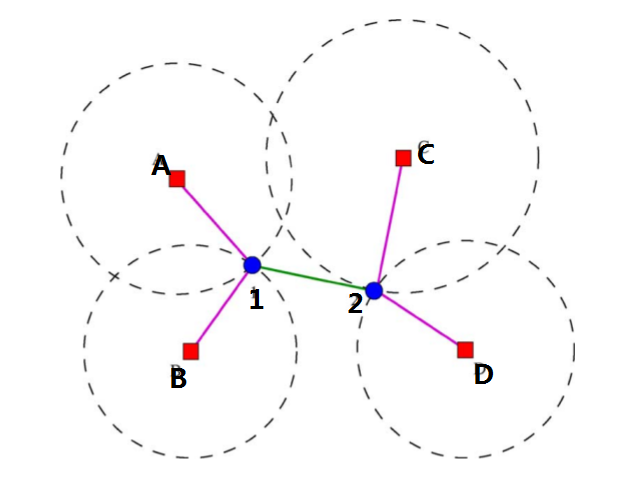
\includegraphics[width=\textwidth]{003.png}
\end{figure}

有些移动节点之前可以相互通信进行相对测距,假设第i和第j个移动节点之间进行测距,得到的观测变量服从均值为
$f(||\bm{p}^a_i-\bm{p}^a_j||)$
方差为$\sigma^2$的高斯分布。所有可通信的移动节点的集合记为E,则此种情况下以$N_a$个移动节点位置为待估计参数,联合概率分布具有如下的形式:
\begin{equation}
\prod_{i=1}^{N_a} f(x^i_1,...x^{i}_{N_b}|\bm{p^a_i})\prod_{(i,j)\in E}\frac{1}{\sqrt{2\pi\sigma^2}}exp(-\frac{(x_{ij}-f(||\bm{p}^a_i-\bm{p}^a_j||))^2}{2\sigma^2})
\end{equation}
上式第一项连乘式是$N_b$个锚点的贡献,第二项连乘式是移动节点协作的贡献。仿照上面的思路可以求出此时的FIM具有如下的结构:
\begin{equation}
J(\bm{P})=
\left(
\begin{array}{cccc}
J^A(\bm{p}_1)+&-\bm{C}_{1,2}&...&-\bm{C}_{1,N_a}\\
\sum_{j\in \{1,..N_a\}\backslash\{1\}}\bm{C}_{1,j}&&&\\
&&&\\
-\bm{C}_{1,2} & J^A(\bm{p}_2)+
&...&-\bm{C}_{2,N_a}\\
&\sum_{j\in \{1,..N_a\}\backslash \{2\}}\bm{C}_{2,j}&&\\
...&&...&\\
-\bm{C}_{1,N_a}&-\bm{C}_{2,N_a}&...& J^A(\bm{p}_{N_a})+\sum_{j\in \{1,..N_a\}\backslash\{N_a\}}\bm{C}_{N_a,j}\\
\end{array}
\right)
\end{equation}
上面的式子中$\bm{P}=(\bm{p}_1,\bm{p}_2,...\bm{p}_{N_a})$,$J^A(\bm{p}_i)$表示$N_b$个锚点对移动节点i的贡献,其具有(\ref{eq:uu})的形式。
$C_{i,j}$表示移动节点i和j协作的矩阵,其具有$\bm{1}_{(i,j)\in E}\lambda_{i,j}\bm{u}\bm{u}^T$的形式,u是两个移动节点间的单位方向向量,如果i,j之间没有通信,该位置为全零的2阶方阵。
$N_a \backslash \{i\}$应理解为移动节点序号1到$N_a$中去掉i后的集合。
相比起非协作的情形,协作定位的FIM存在耦合项,即非对角元非零的情况,因而其FIM的结构更复杂。通过简单的观察,我们发现$J(\bm{P})$每一行之和和非协作时相等,都严格大于0,这种严格对角占优的性质能否在之后的研究中利用上也是一个可以探讨的话题。
FIM和协方差矩阵的关系,(\ref{eq:uu})式可以看成如下随机变量的方差:
\begin{equation}
X=\sum_{i=1}^{N_b} \frac{(X_i-f(||\bm{p}^b_i-\bm{p}||))\times f'}{\sqrt{2}\sigma^2}(\bm{p}^b_i-\bm{p})
\end{equation}
X是$X_i$的线性组合,由$X_i$之间的独立性很容易求出
$D(X)=FIM(\ref{eq:uu})$
这种构造可以推广到$N_a$个移动节点的情形,此时
\begin{equation}
X^a_j=\sum_{i=1}^{N_b} \frac{(X_{i,j}-f(||\bm{p}^b_i-\bm{p}^a_j||))\times f'}{\sqrt{2}\sigma^2}(\bm{p}^b_i-\bm{p}^a_j)
\end{equation}
上式j取1,2,...$N_a$,$X_{a,i}$表示第i个锚点和第j个移动节点测距的正态随机变量,由$X_{a,i}$的彼此独立性可以推出协方差阵$Corr(\bm{X})$为由(\ref{eq:uu})组成的对角阵,其中$\bm{X}=(X^a_1,X^a_2,...X^a_{N_a})$
考虑节点的相互协作后,每一个$X^a_j$附加了协作项
\begin{equation}
X^a_j=X^a_j(\text{non coorperative})+\sum_{(j,i)\in E}\frac{(X_{ij}-f(||\bm{p}^a_i-\bm{p}^a_j||))\times f'}{\sqrt{2}\sigma^2}(\bm{p}^a_i-\bm{p}^a_j)
\end{equation}
上式$X_{ij}$表示移动节点i和j协作测距的正态随机变量。由上式求$\bm{X}$的协方差矩阵可以得到$J(\bm{P})$.因此对每一个移动节点我们分配了一个随机变量$X^a_j$,目标是研究$X^a_j$之间的关系,可以用主成分分析或者因子分析的方法。

\end{document}